\documentclass{report}

\usepackage{hyperref}

\usepackage{epstopdf}
\usepackage{amsmath}
\usepackage{amssymb}
\usepackage{subfig}
%\usepackage{multirow}
\usepackage[utf8]{inputenc}
\usepackage[T1]{fontenc}
\usepackage{standalone}
\usepackage{tikz}
\usepackage{tabularx}
\usepackage{float}
\usepackage[section]{placeins}
\usepackage{sverb}
\usepackage{import}
\usepackage{verbatim}
\usepackage{listings}
\usepackage{xcolor}

\graphicspath{{img/}}
\DeclareGraphicsExtensions{.pdf,.png,.jpg,.svg} %For pdflatex






\begin{document}

\begin{titlepage}
    \begin{center}
        
\includegraphics[width=.50\linewidth]{other/polsl.png}\\
        \Huge
        \textbf{Przetwarzanie Obrazów Cyfrowych}
        \\ \vspace{1.5cm}
        \Large
        \textbf{Raport z ćwiczenia nr. 6: } \\
        % \textbf{WSTĘPNE PRZETWARZANIE OBRAZÓW — FILTRY LINIOWE}
        \textbf{Wstępne przetwarzanie obrazów - filtry liniowe}        
    \end{center}
    \vspace{3.0cm}
    \Large
    Raport opracował: \\
    Dawid Kania \\
    Grupa 6 Semestr 6 \\ \\
    Data wykonania ćwiczenia: 09.06.2022
\end{titlepage}
 


\section*{Zadanie 1. Operacje na histogramach}
\subsection*{Rozciąganie histogramu}


\newcommand{\ww}{0.33}
\begin{figure}[H]
    \captionsetup[subfloat]{justification=raggedright,singlelinecheck=false, position=bottom,labelformat=empty} %
    \subfloat[]{\includegraphics[width=\ww\linewidth]{../zad1/NoCut/I1/I_Origin.png}} \hfill%	
    \subfloat[]{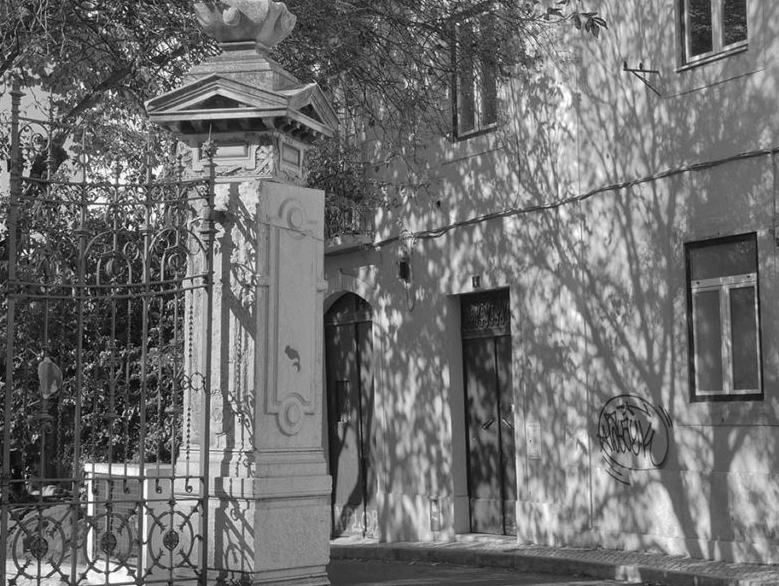
\includegraphics[width=\ww\linewidth]{../zad1/NoCut/I1/I_No_Cut.png}} \hfill% wypełnenie
    \subfloat[]{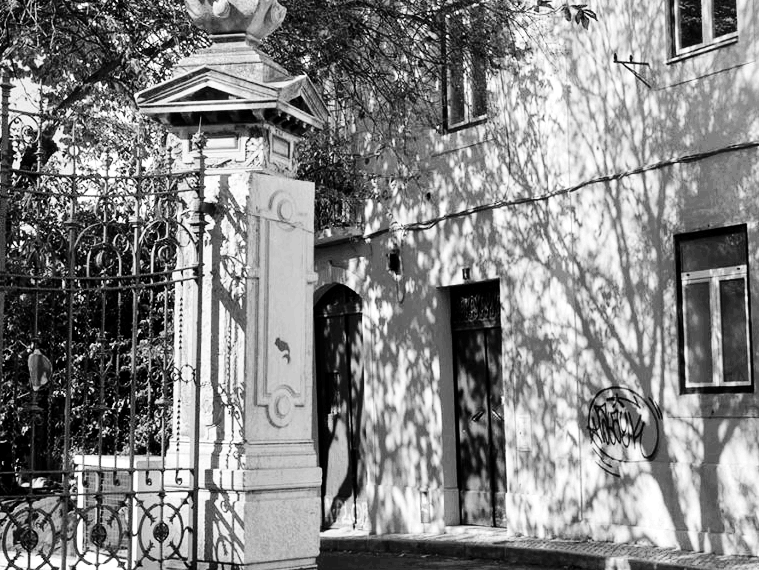
\includegraphics[width=\ww\linewidth]{../zad1/NoCut/I1/I_Histeq.png}} \\
    \subfloat[k1 = 0.28627 \\ k2 = 2.3275 \\ k3 = 1 \\ k4 = 0.010884 \\ min(I) = 0 \\ max(I) = 0.28627 ]{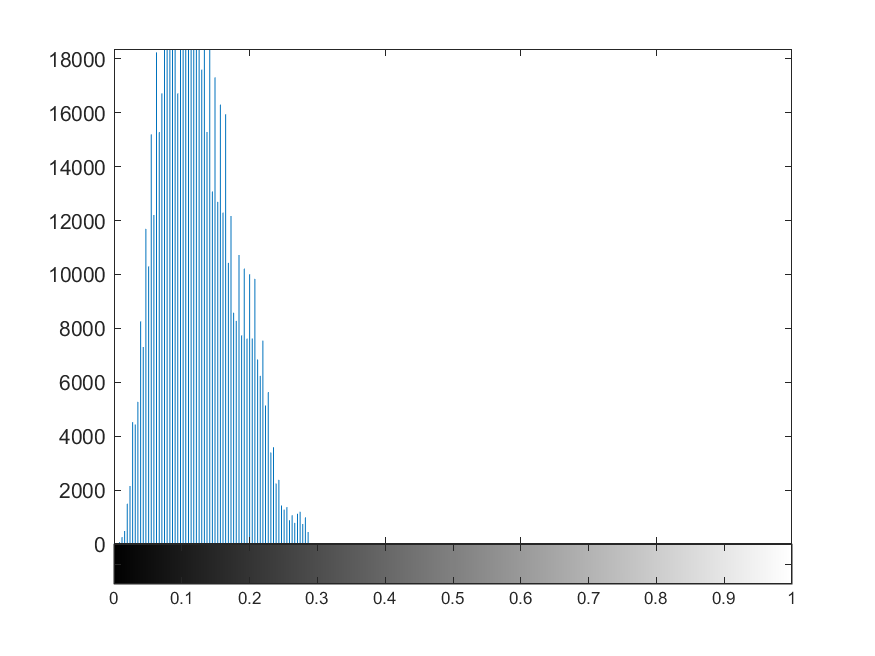
\includegraphics[width=\ww\linewidth]{../zad1/NoCut/I1/H_Origin.png}} \hfill%	
    \subfloat[k1 = 1 \\ k2 = 2.3275 \\ k3 = 1 \\ k4 = 0.13281 \\ min(I) = 0 \\ max(I) = 1 ]{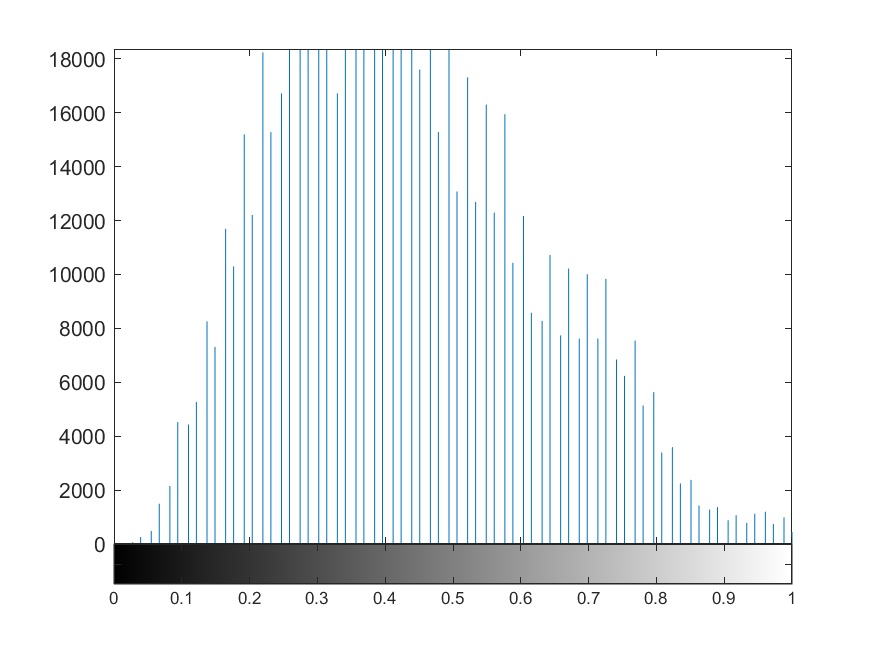
\includegraphics[width=\ww\linewidth]{../zad1/NoCut/I1/H_No_Cut.png}} \hfill
    \subfloat[k1 = 1 \\ k2 = 2.0034 \\ k3 = 1 \\ k4 = 0.34362 \\ min(I) = 0 \\ max(I) = 1 ]{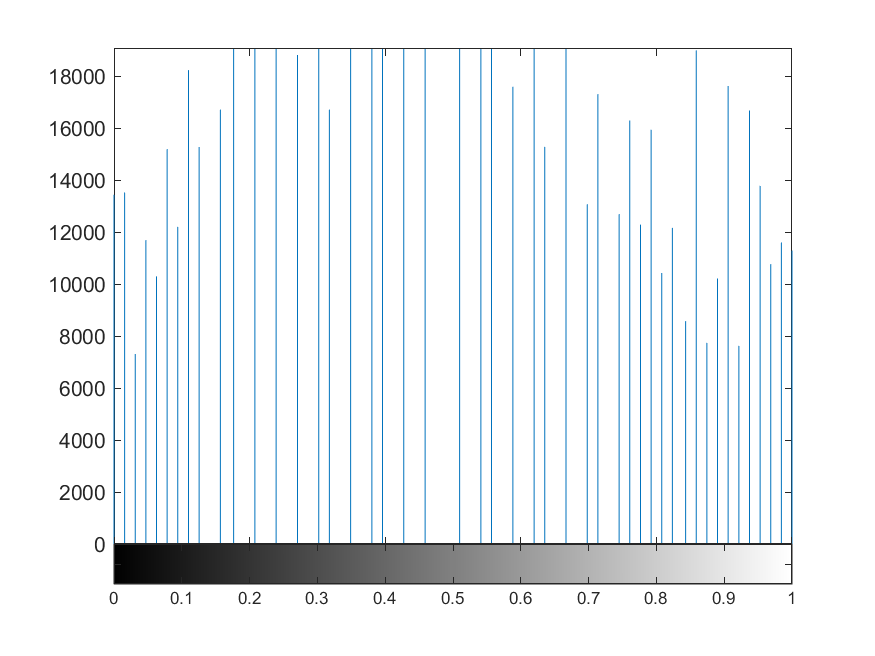
\includegraphics[width=\ww\linewidth]{../zad1/NoCut/I1/H_Histeq.png}} 
    \caption{Tekst do zmiany} 
    \label{fig:porownanie1}
\end{figure}

\begin{figure}[H]
    \captionsetup[subfloat]{justification=raggedright,singlelinecheck=false, position=bottom,labelformat=empty} %
    \subfloat[]{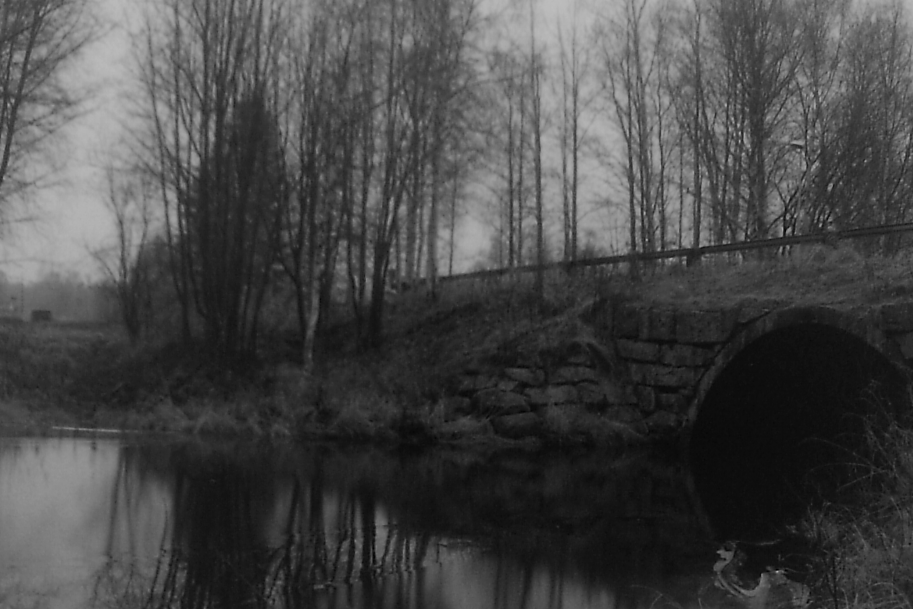
\includegraphics[width=\ww\linewidth]{../zad1/NoCut/I2/I_Origin.png}} \hfill%	
    \subfloat[]{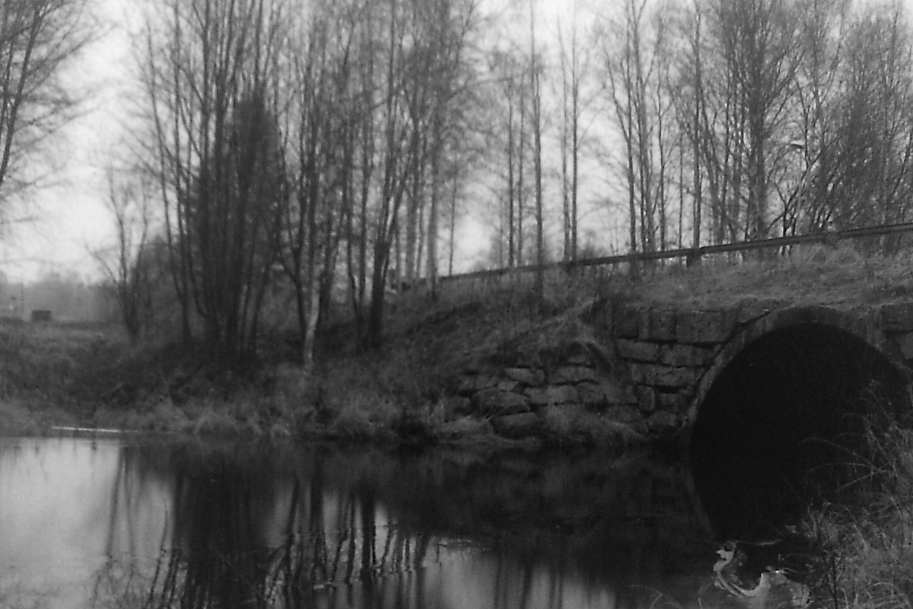
\includegraphics[width=\ww\linewidth]{../zad1/NoCut/I2/I_No_Cut.png}} \hfill% wypełnenie
    \subfloat[]{\includegraphics[width=\ww\linewidth]{../zad1/NoCut/I2/I_Histeq.png}} \\
    \subfloat[k1 = 0.76078 \\ k2 = 2.4201 \\ k3 = 1 \\ k4 = 0.15035 \\ min(I) = 0 \\ max(I) = 0.76078 ]{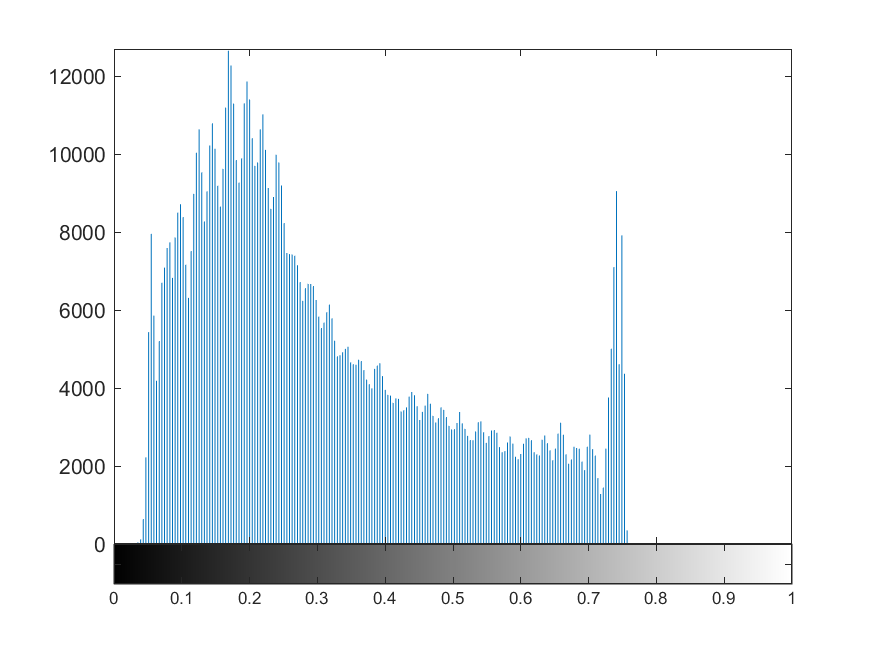
\includegraphics[width=\ww\linewidth]{../zad1/NoCut/I2/H_Origin.png}} \hfill%	
    \subfloat[k1 = 1 \\ k2 = 2.4201 \\ k3 = 1 \\ k4 = 0.25977 \\ min(I) = 0 \\ max(I) = 1 ]{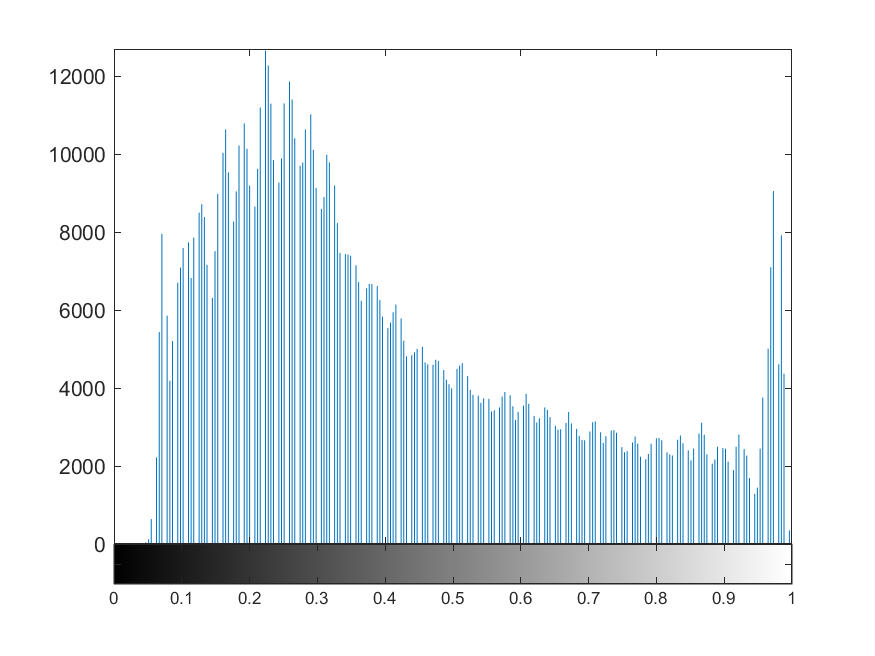
\includegraphics[width=\ww\linewidth]{../zad1/NoCut/I2/H_No_Cut.png}} \hfill
    \subfloat[k1 = 1 \\ k2 = 2.001 \\ k3 = 1 \\ k4 = 0.34525 \\ min(I) = 0 \\ max(I) = 1 ]{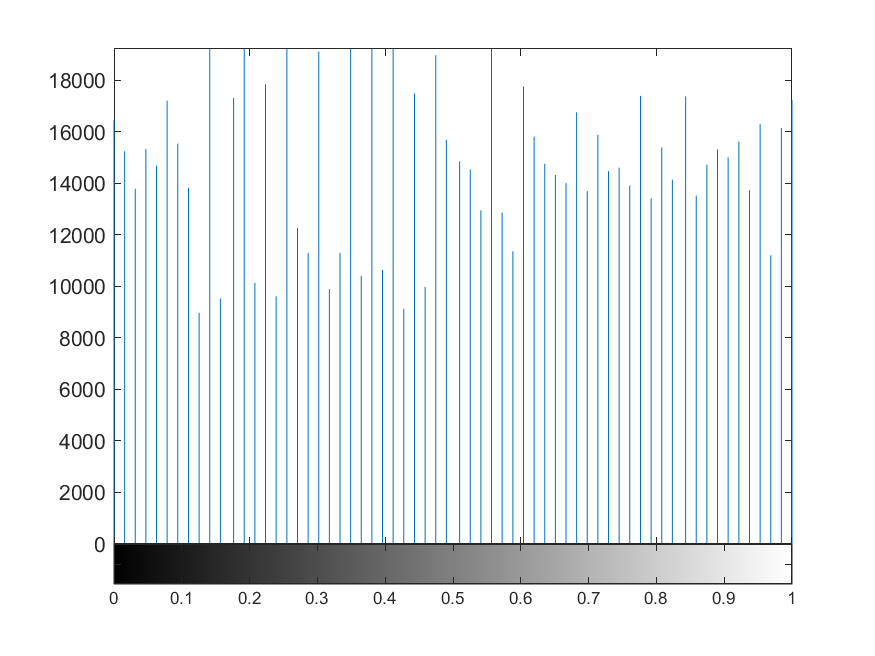
\includegraphics[width=\ww\linewidth]{../zad1/NoCut/I2/H_Histeq.png}} 
    \caption{Tekst do zmiany} 
    \label{fig:porownanie2}
\end{figure}

\begin{figure}[H]
    \captionsetup[subfloat]{justification=raggedright,singlelinecheck=false, position=bottom,labelformat=empty} %
    \subfloat[]{\includegraphics[width=\ww\linewidth]{../zad1/NoCut/I3/I_Origin.png}} \hfill%	
    \subfloat[]{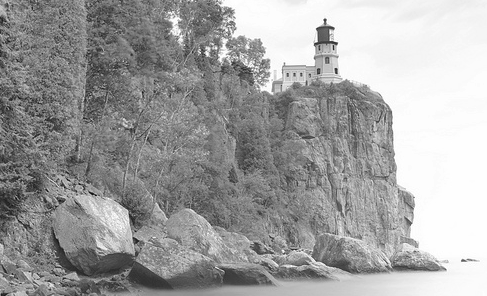
\includegraphics[width=\ww\linewidth]{../zad1/NoCut/I3/I_No_Cut.png}} \hfill% wypełnenie
    \subfloat[]{\includegraphics[width=\ww\linewidth]{../zad1/NoCut/I3/I_Histeq.png}} \\
    \subfloat[k1 = 0.81961 \\ k2 = 1.479 \\ k3 = 1 \\ k4 = 0.16253 \\ min(I) = 0 \\ max(I) = 0.81961 ]{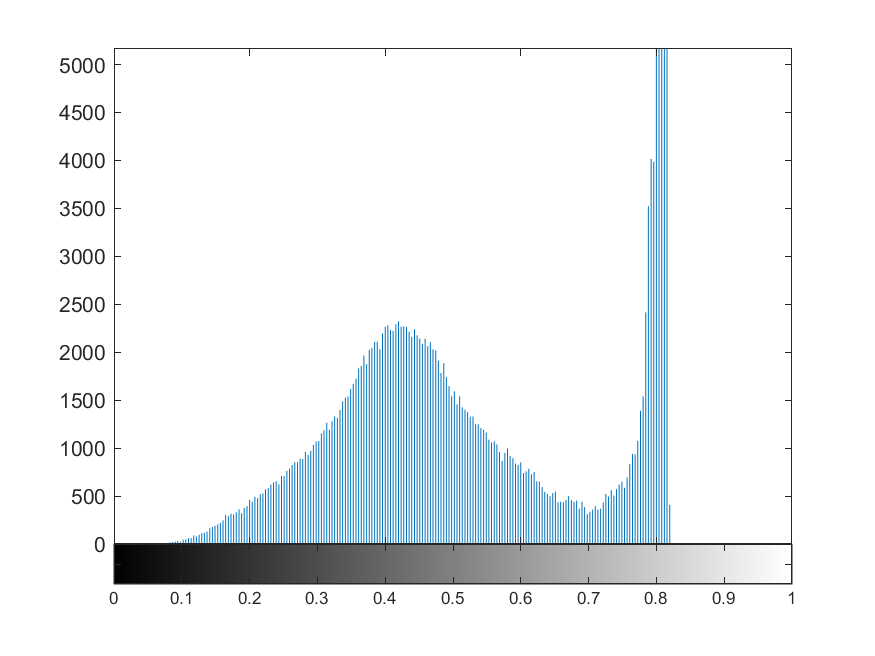
\includegraphics[width=\ww\linewidth]{../zad1/NoCut/I3/H_Origin.png}} \hfill%	
    \subfloat[k1 = 1 \\ k2 = 1.479 \\ k3 = 1 \\ k4 = 0.24194 \\ min(I) = 0 \\ max(I) = 1 ]{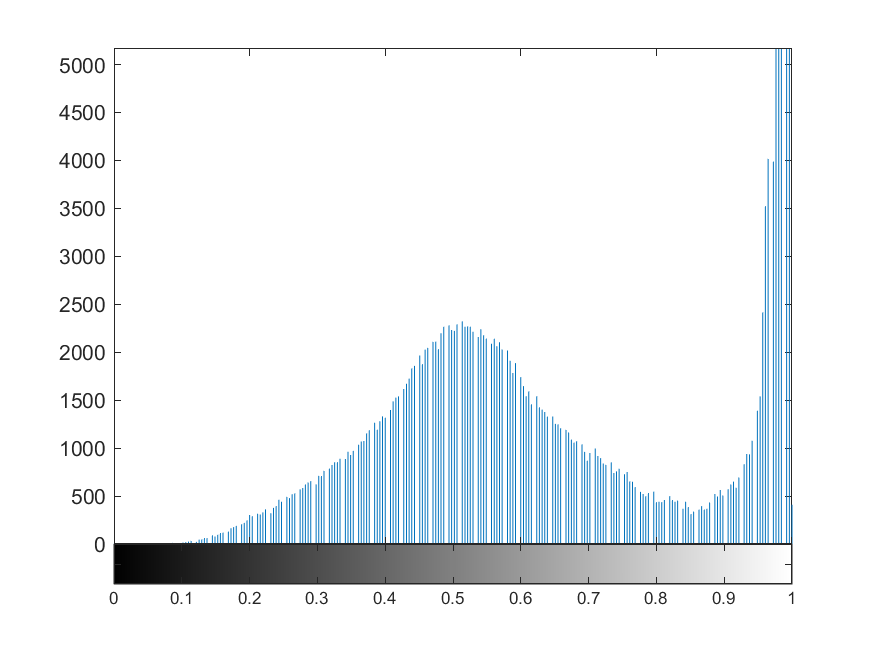
\includegraphics[width=\ww\linewidth]{../zad1/NoCut/I3/H_No_Cut.png}} \hfill
    \subfloat[k1 = 1 \\ k2 = 1.9995 \\ k3 = 1 \\ k4 = 0.34542 \\ min(I) = 0 \\ max(I) = 1 ]{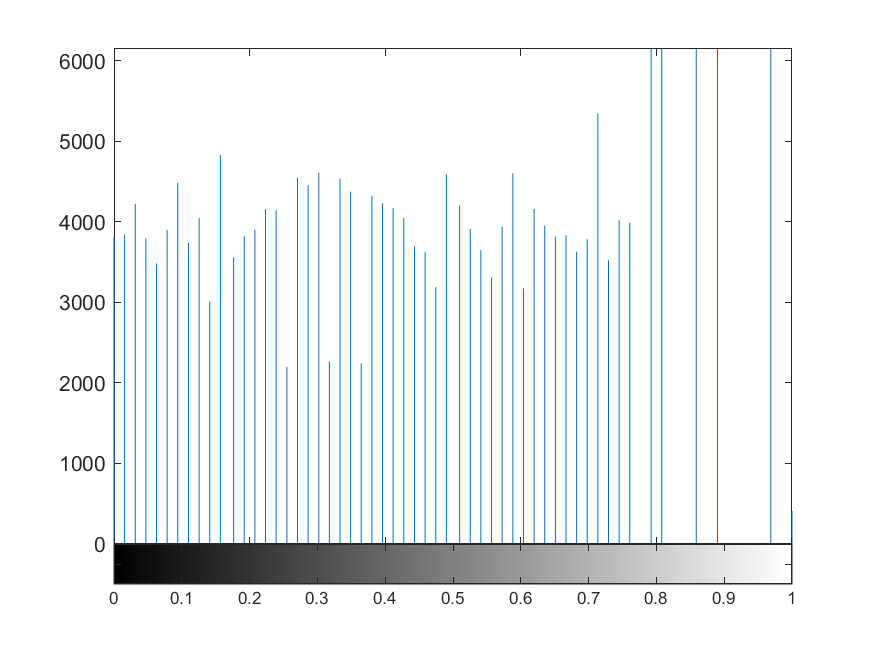
\includegraphics[width=\ww\linewidth]{../zad1/NoCut/I3/H_Histeq.png}} 
    \caption{Tekst do zmiany} 
    \label{fig:porownanie3}
\end{figure}

\begin{figure}[H]
    \captionsetup[subfloat]{justification=raggedright,singlelinecheck=false, position=bottom,labelformat=empty} %
    \subfloat[]{\includegraphics[width=\ww\linewidth]{../zad1/NoCut/I4/I_Origin.png}} \hfill%	
    \subfloat[]{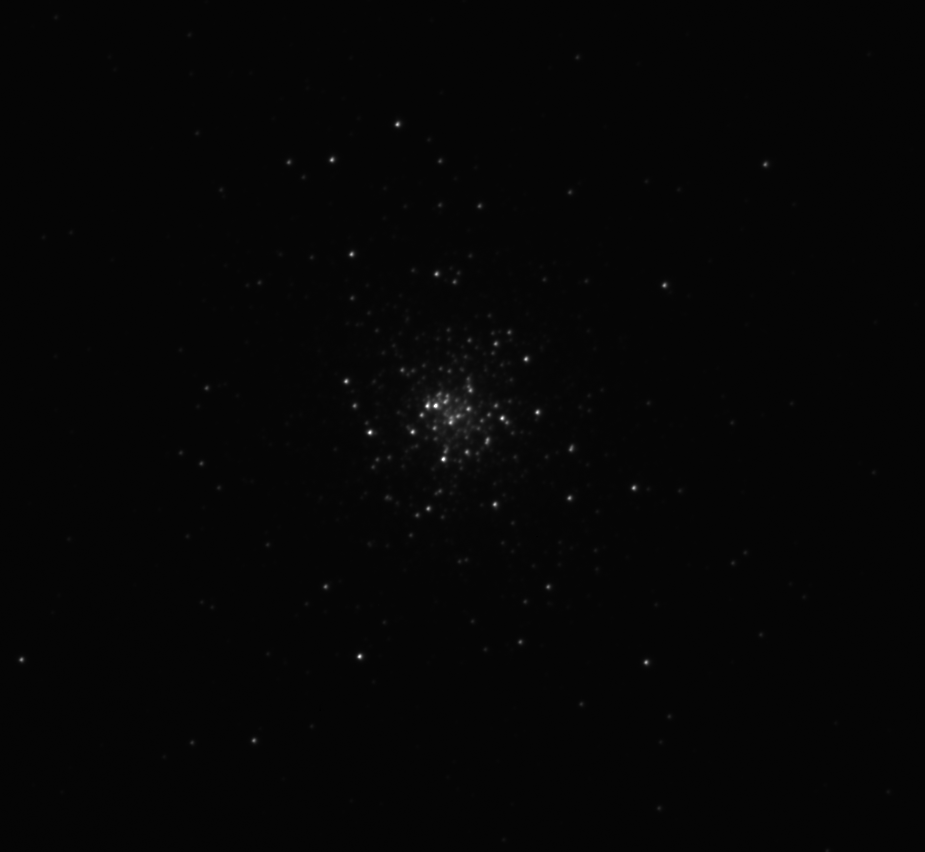
\includegraphics[width=\ww\linewidth]{../zad1/NoCut/I4/I_No_Cut.png}} \hfill% wypełnenie
    \subfloat[]{\includegraphics[width=\ww\linewidth]{../zad1/NoCut/I4/I_Histeq.png}} \\
    \subfloat[k1 = 0.28627 \\ k2 = 2.3275 \\ k3 = 1 \\ k4 = 0.010884 \\ min(I) = 0 \\ max(I) = 0.28627 ]{\includegraphics[width=\ww\linewidth]{../zad1/NoCut/I4/H_Origin.png}} \hfill%	
    \subfloat[k1 = 1 \\ k2 = 2.3275 \\ k3 = 1 \\ k4 = 0.13281 \\ min(I) = 0 \\ max(I) = 1 ]{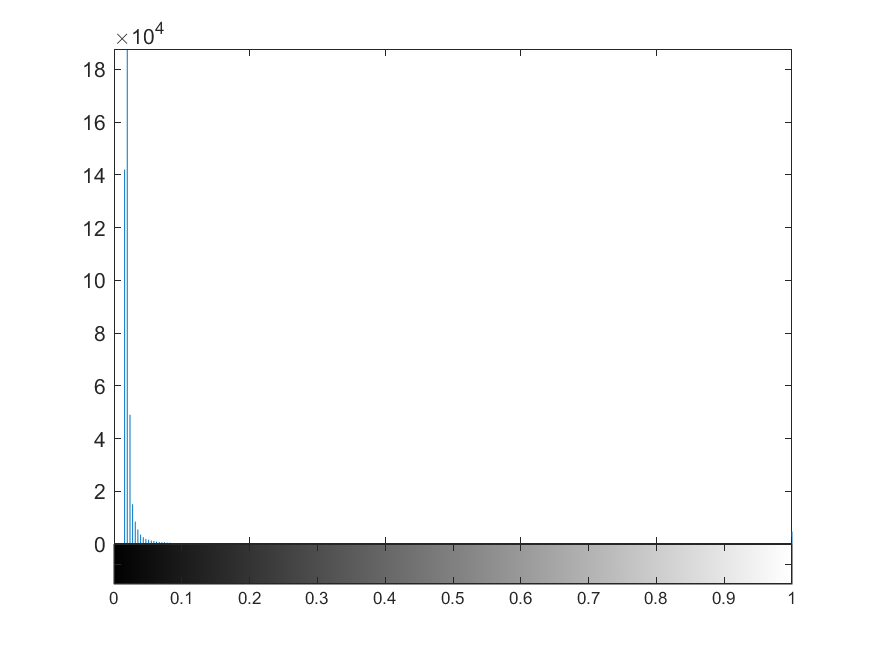
\includegraphics[width=\ww\linewidth]{../zad1/NoCut/I4/H_No_Cut.png}} \hfill
    \subfloat[k1 = 1 \\ k2 = 2.0034 \\ k3 = 1 \\ k4 = 0.34362 \\ min(I) = 0 \\ max(I) = 1 ]{\includegraphics[width=\ww\linewidth]{../zad1/NoCut/I4/H_Histeq.png}} 
    \caption{Tekst do zmiany} 
    \label{fig:porownanie4}
\end{figure}



\subsection*{Rozciąganie histogramu z obcinaniem}

\begin{figure}[H]
    \captionsetup[subfloat]{justification=raggedright,singlelinecheck=false, position=bottom,labelformat=empty} %
    \subfloat[]{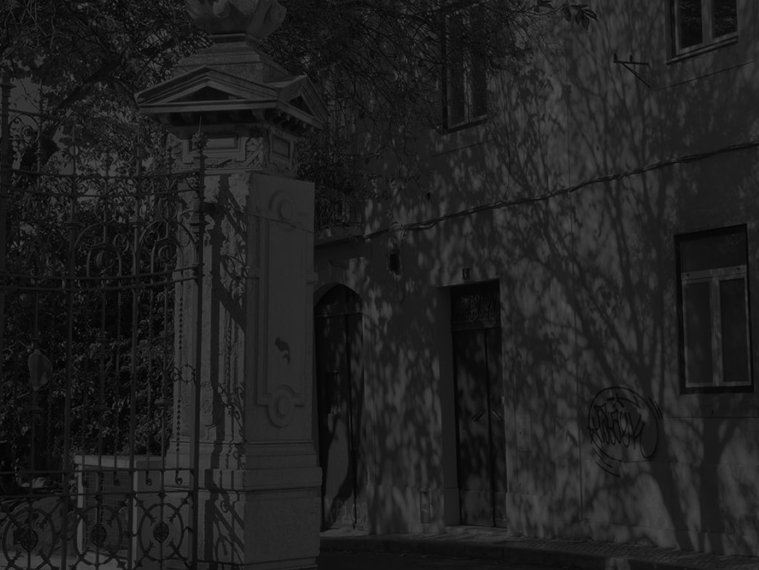
\includegraphics[width=\ww\linewidth]{../zad1/WithCut/I1/I_Origin.png}} \hfill%	
    \subfloat[]{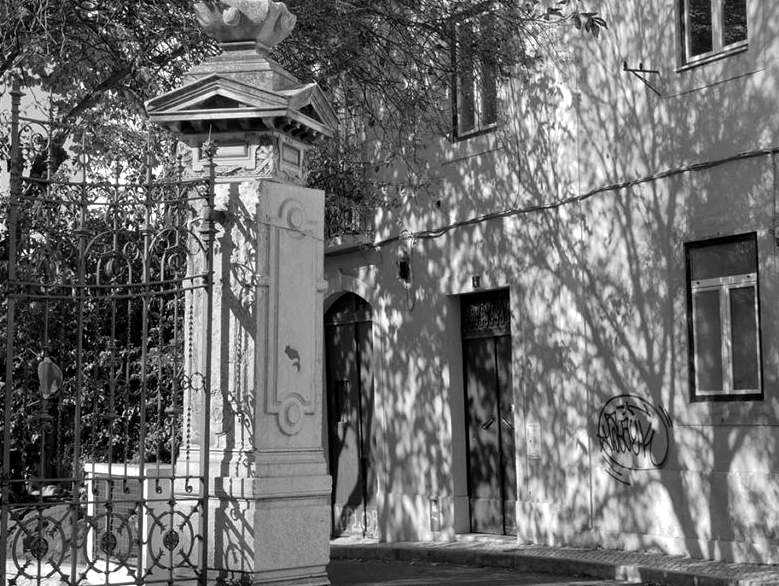
\includegraphics[width=\ww\linewidth]{../zad1/WithCut/I1/I_No_Cut.png}} \hfill% wypełnenie
    \subfloat[]{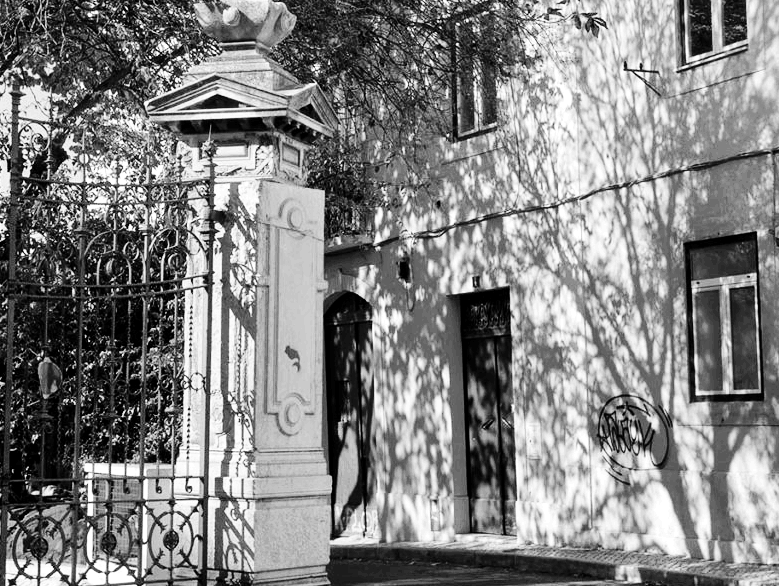
\includegraphics[width=\ww\linewidth]{../zad1/WithCut/I1/I_Histeq.png}} \\
    \subfloat[k1 = 1 \\ k2 = 8.1303 \\ k3 = 1 \\ k4 = 0.010888 \\ min(I) = 0 \\ max(I) = 1 ]{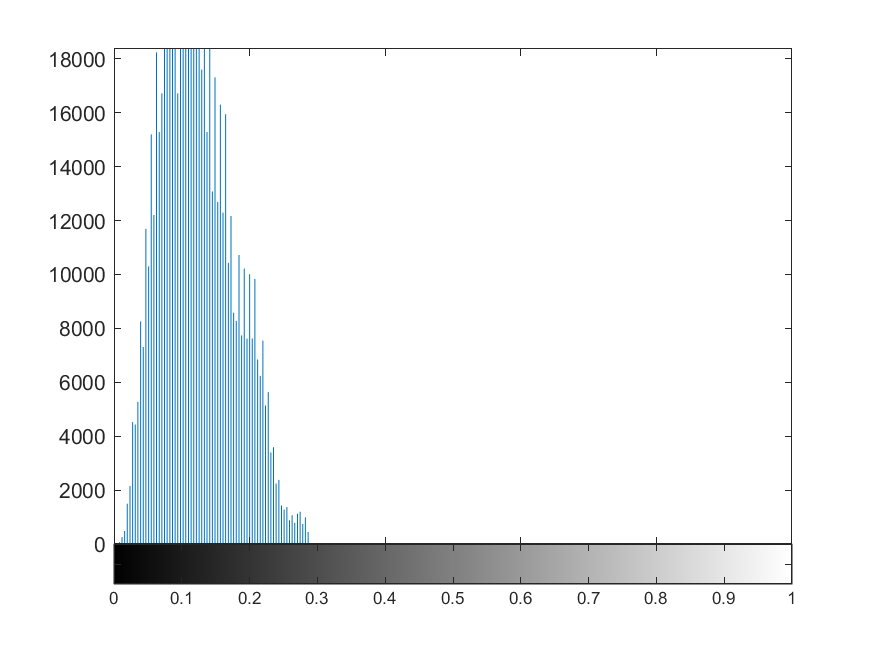
\includegraphics[width=\ww\linewidth]{../zad1/WithCut/I1/H_Origin.png}} \hfill%	
    \subfloat[k1 = 1 \\ k2 = 2.3834 \\ k3 = 1 \\ k4 = 0.20638 \\ min(I) = 0 \\ max(I) = 1 ]{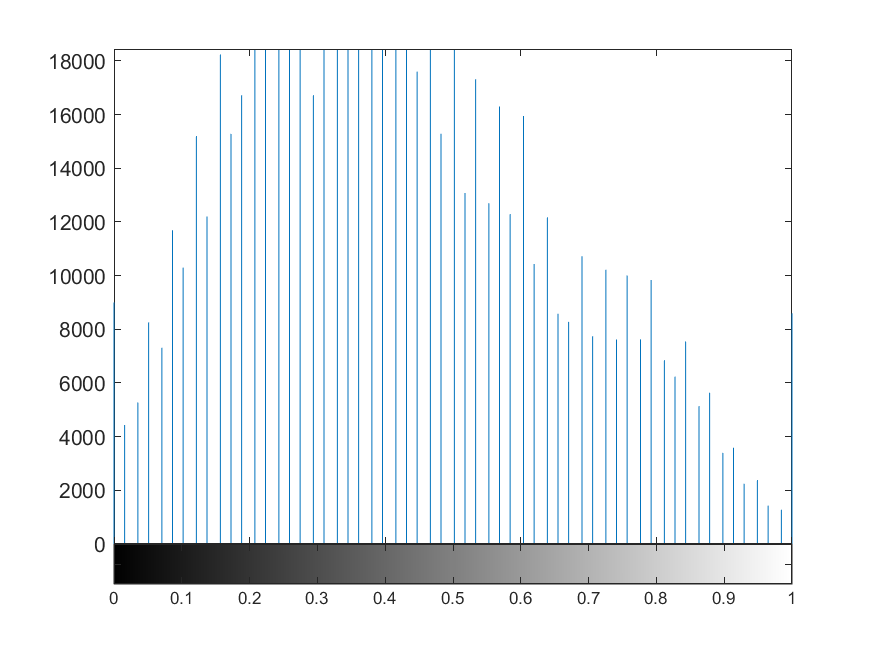
\includegraphics[width=\ww\linewidth]{../zad1/WithCut/I1/H_No_Cut.png}} \hfill
    \subfloat[k1 = 1 \\ k2 = 2.0034 \\ k3 = 1 \\ k4 = 0.34362 \\ min(I) = 0 \\ max(I) = 1 ]{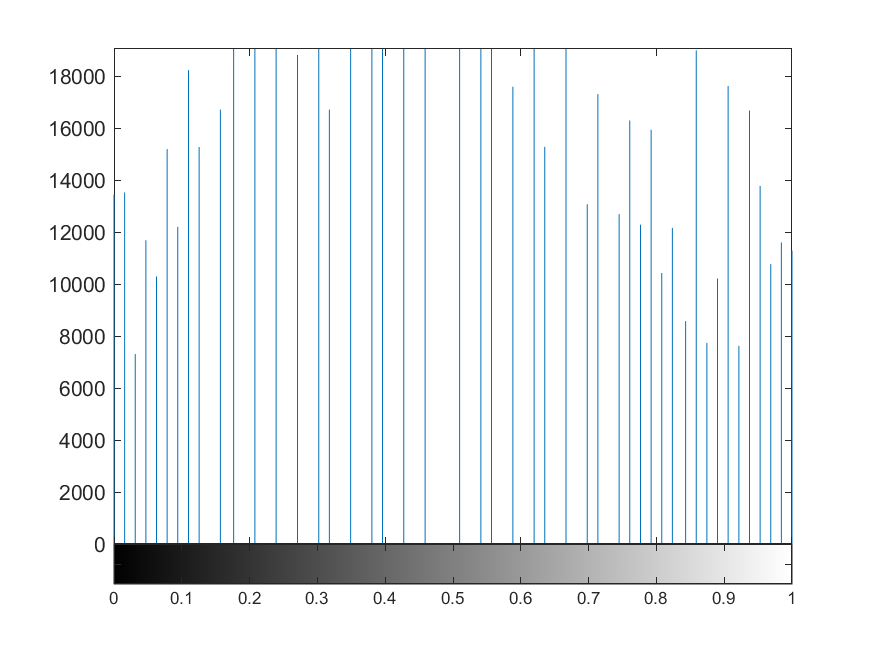
\includegraphics[width=\ww\linewidth]{../zad1/WithCut/I1/H_Histeq.png}} 
    \caption{Tekst do zmiany} 
    \label{fig:porownanie5}
\end{figure}

\begin{figure}[H]
    \captionsetup[subfloat]{justification=raggedright,singlelinecheck=false, position=bottom,labelformat=empty} %
    \subfloat[]{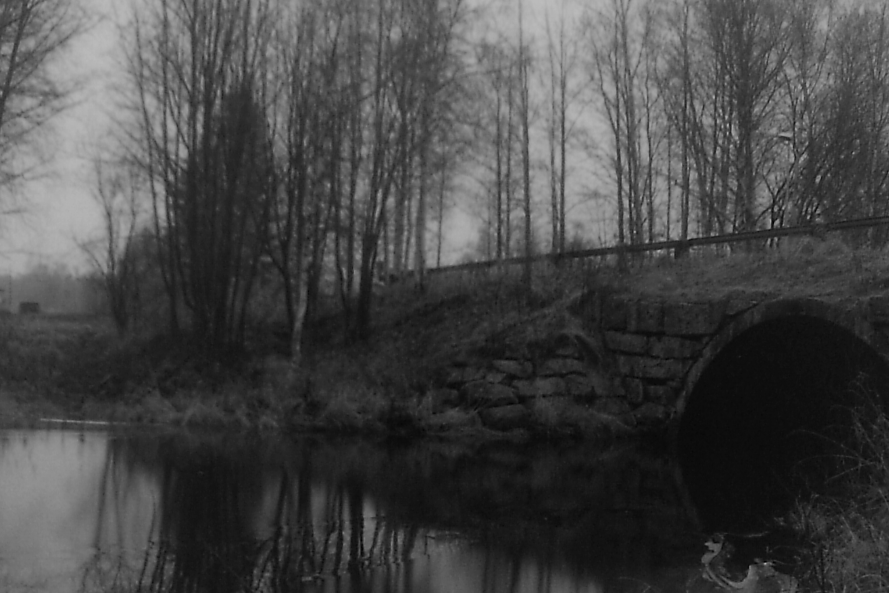
\includegraphics[width=\ww\linewidth]{../zad1/WithCut/I2/I_Origin.png}} \hfill%	
    \subfloat[]{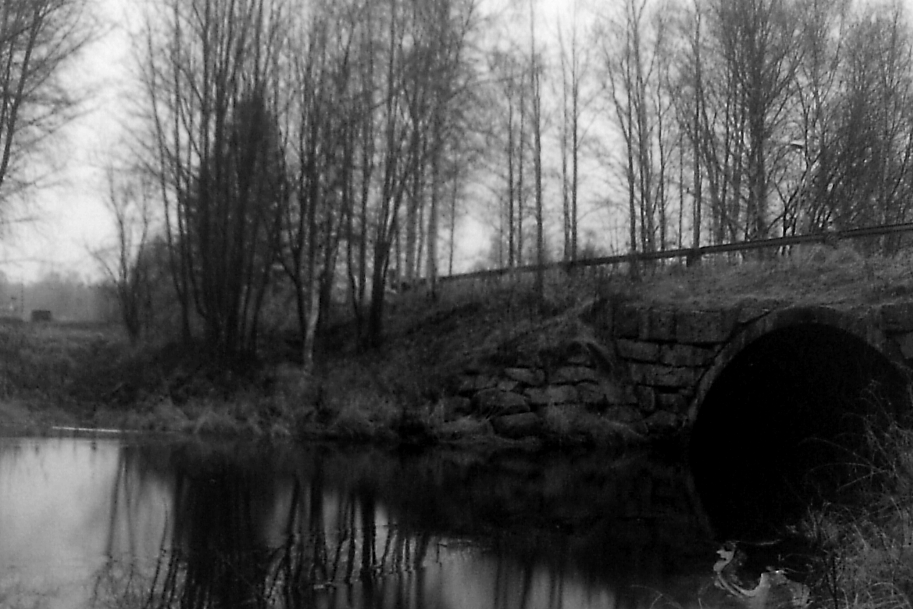
\includegraphics[width=\ww\linewidth]{../zad1/WithCut/I2/I_No_Cut.png}} \hfill% wypełnenie
    \subfloat[]{\includegraphics[width=\ww\linewidth]{../zad1/WithCut/I2/I_Histeq.png}} \\
    \subfloat[k1 = 1 \\ k2 = 3.181 \\ k3 = 1 \\ k4 = 0.15035 \\ min(I) = 0 \\ max(I) = 1 ]{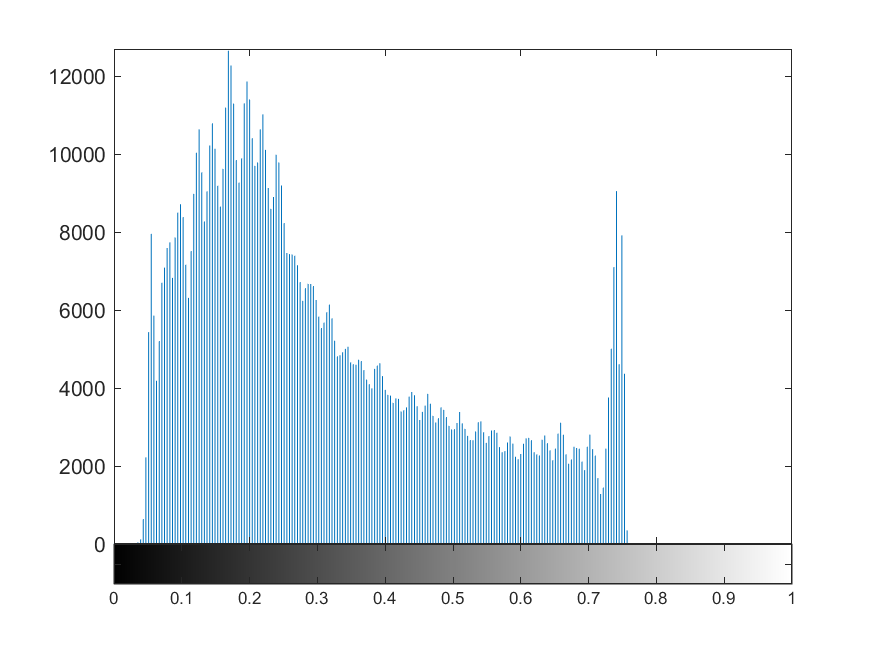
\includegraphics[width=\ww\linewidth]{../zad1/WithCut/I2/H_Origin.png}} \hfill%	
    \subfloat[k1 = 1 \\ k2 = 2.6749 \\ k3 = 1 \\ k4 = 0.31169 \\ min(I) = 0 \\ max(I) = 1 ]{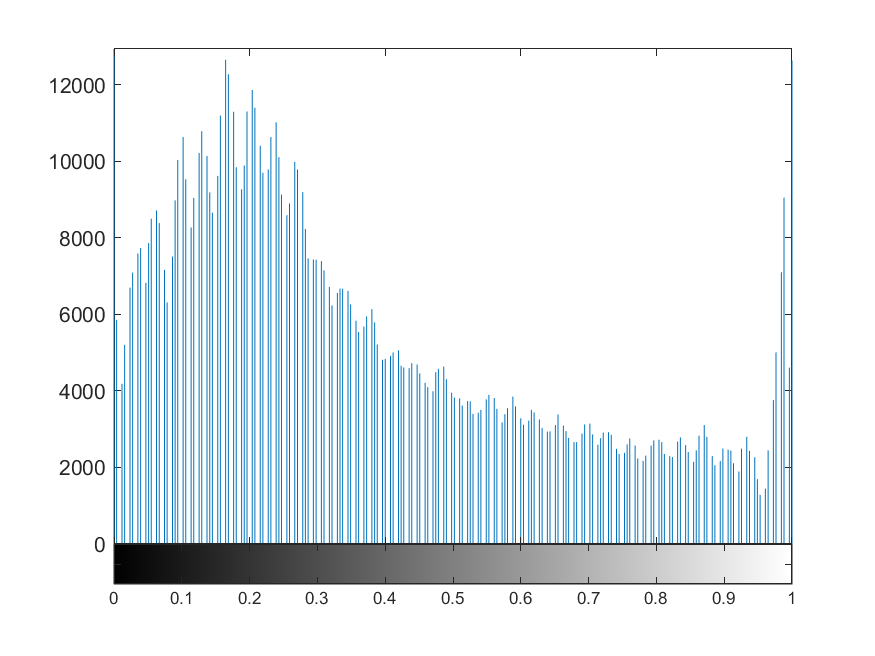
\includegraphics[width=\ww\linewidth]{../zad1/WithCut/I2/H_No_Cut.png}} \hfill
    \subfloat[k1 = 1 \\ k2 = 2.001 \\ k3 = 1 \\ k4 = 0.34525 \\ min(I) = 0 \\ max(I) = 1 ]{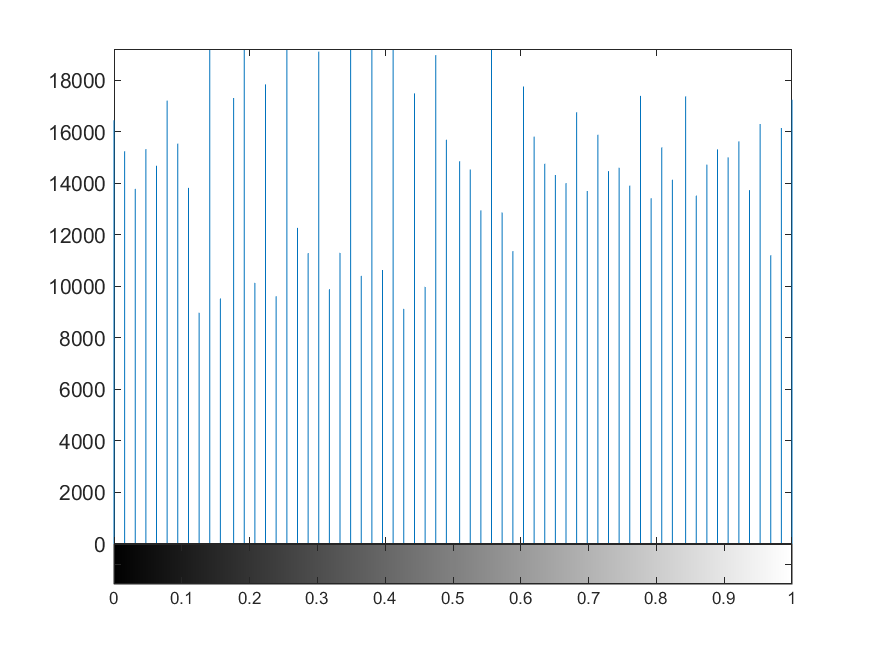
\includegraphics[width=\ww\linewidth]{../zad1/WithCut/I2/H_Histeq.png}} 
    \caption{Tekst do zmiany} 
    \label{fig:porownanie6}
\end{figure}

\begin{figure}[H]
    \captionsetup[subfloat]{justification=raggedright,singlelinecheck=false, position=bottom,labelformat=empty} %
    \subfloat[]{\includegraphics[width=\ww\linewidth]{../zad1/WithCut/I3/I_Origin.png}} \hfill%	
    \subfloat[]{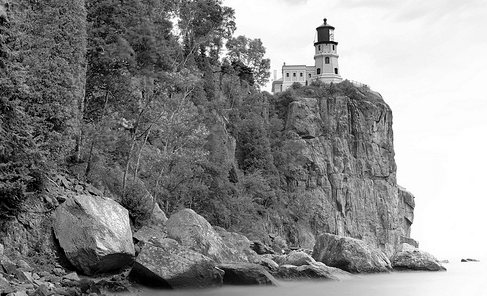
\includegraphics[width=\ww\linewidth]{../zad1/WithCut/I3/I_No_Cut.png}} \hfill% wypełnenie
    \subfloat[]{\includegraphics[width=\ww\linewidth]{../zad1/WithCut/I3/I_Histeq.png}} \\
    \subfloat[k1 = 1 \\ k2 = 1.8045 \\ k3 = 1 \\ k4 = 0.16253 \\ min(I) = 0 \\ max(I) = 1 ]{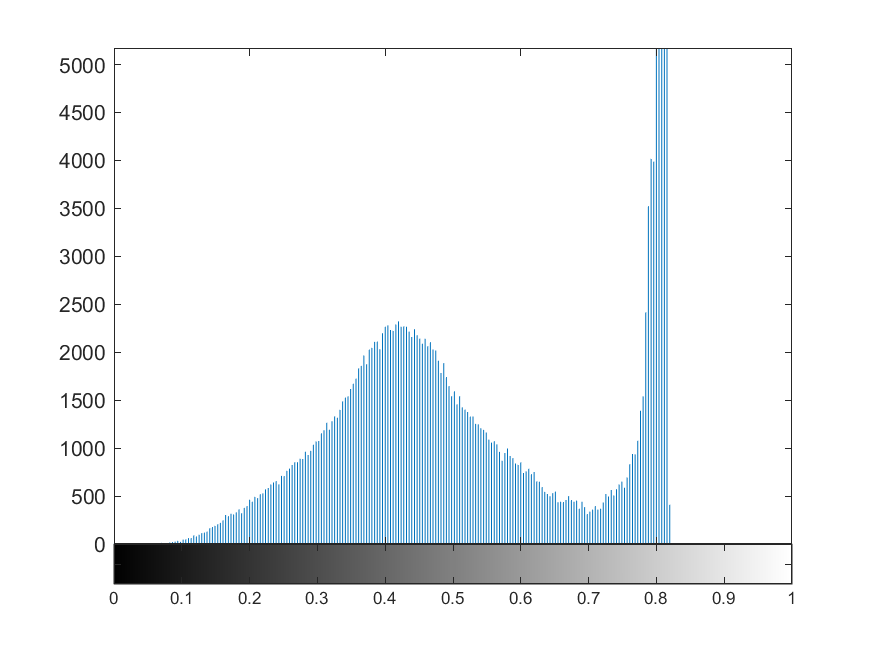
\includegraphics[width=\ww\linewidth]{../zad1/WithCut/I3/H_Origin.png}} \hfill%	
    \subfloat[k1 = 1 \\ k2 = 1.6703 \\ k3 = 1 \\ k4 = 0.38128 \\ min(I) = 0 \\ max(I) = 1 ]{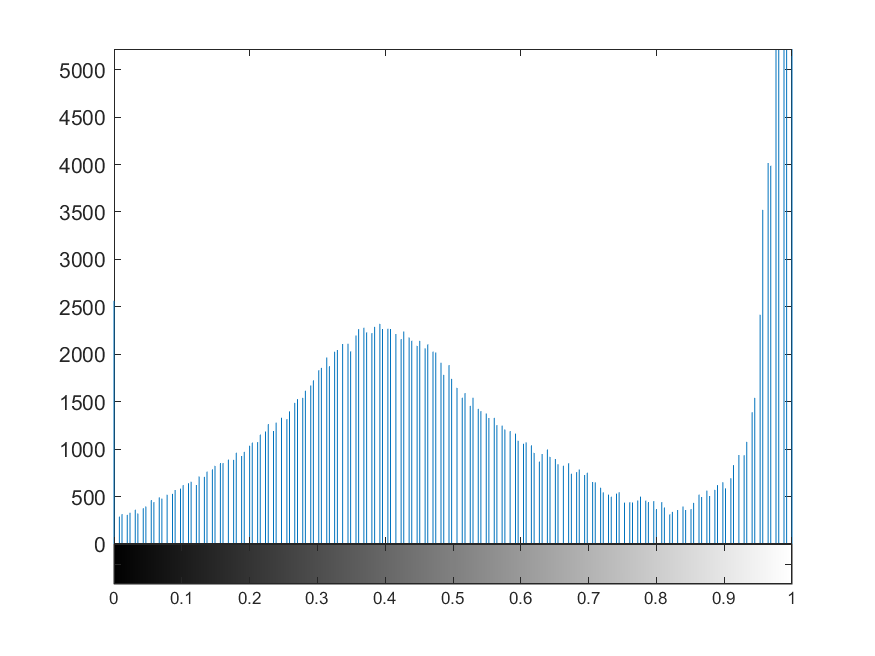
\includegraphics[width=\ww\linewidth]{../zad1/WithCut/I3/H_No_Cut.png}} \hfill
    \subfloat[k1 = 1 \\ k2 = 1.9995 \\ k3 = 1 \\ k4 = 0.34542 \\ min(I) = 0 \\ max(I) = 1 ]{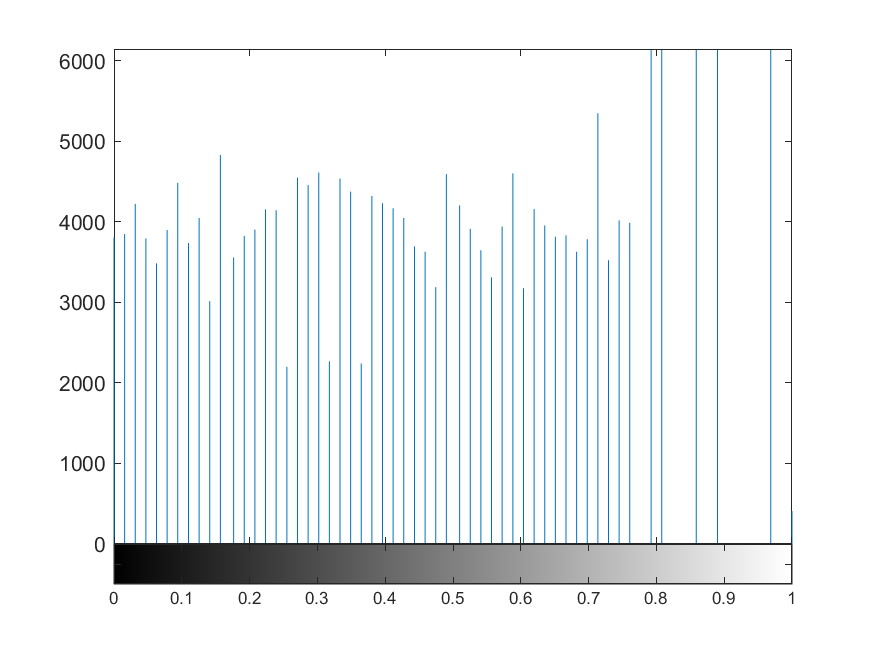
\includegraphics[width=\ww\linewidth]{../zad1/WithCut/I3/H_Histeq.png}} 
    \caption{Tekst do zmiany} 
    \label{fig:porownanie7}
\end{figure}

\begin{figure}[H]
    \captionsetup[subfloat]{justification=raggedright,singlelinecheck=false, position=bottom,labelformat=empty} %
    \subfloat[]{\includegraphics[width=\ww\linewidth]{../zad1/WithCut/I4/I_Origin.png}} \hfill%	
    \subfloat[]{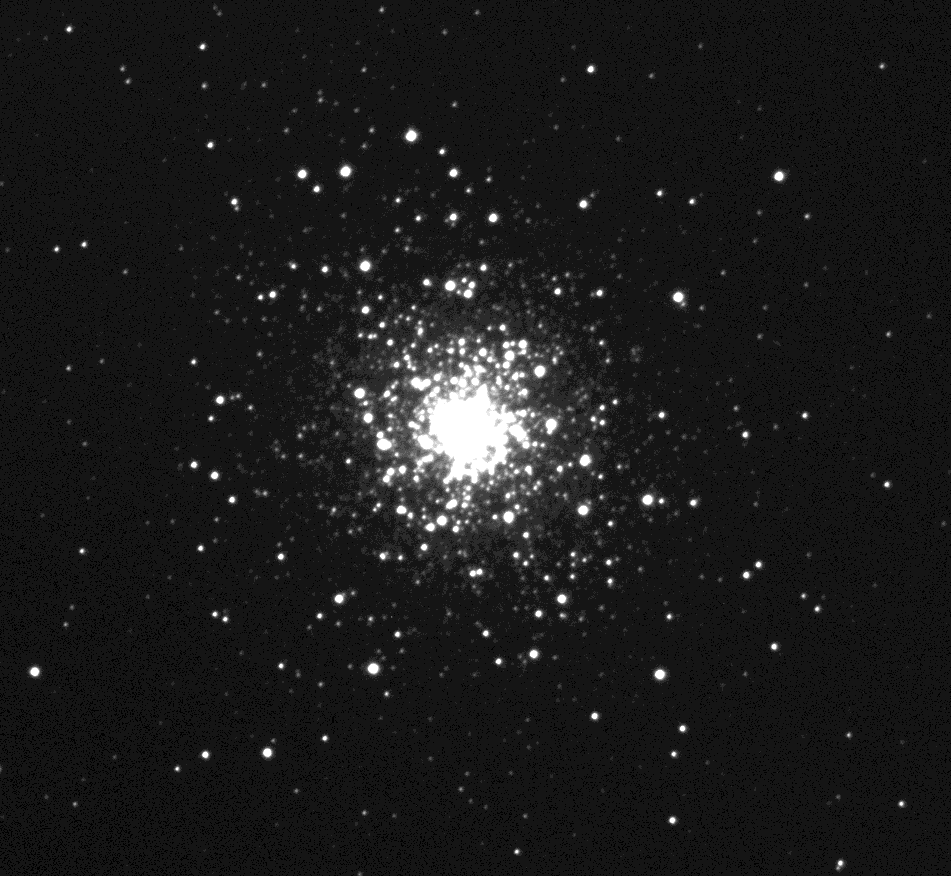
\includegraphics[width=\ww\linewidth]{../zad1/WithCut/I4/I_No_Cut.png}} \hfill% wypełnenie
    \subfloat[]{\includegraphics[width=\ww\linewidth]{../zad1/WithCut/I4/I_Histeq.png}} \\
    \subfloat[k1 = 1 \\ k2 = 31.566 \\ k3 = 1 \\ k4 = 0.013199 \\ min(I) = 0 \\ max(I) = 1 ]{\includegraphics[width=\ww\linewidth]{../zad1/WithCut/I4/H_Origin.png}} \hfill%	
    \subfloat[k1 = 1 \\ k2 = 10.334 \\ k3 = 1 \\ k4 = 0.053819 \\ min(I) = 0 \\ max(I) = 1 ]{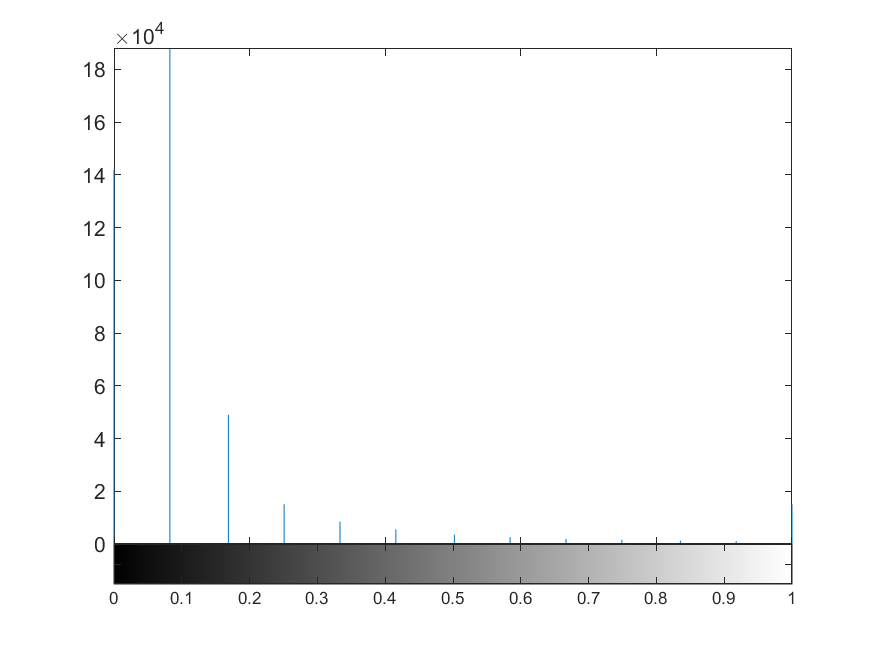
\includegraphics[width=\ww\linewidth]{../zad1/WithCut/I4/H_No_Cut.png}} \hfill
    \subfloat[k1 = 1 \\ k2 = 2.0148 \\ k3 = 1 \\ k4 = 0.14579 \\ min(I) = 0 \\ max(I) = 1 ]{\includegraphics[width=\ww\linewidth]{../zad1/WithCut/I4/H_Histeq.png}} 
    \caption{Tekst do zmiany} 
    \label{fig:porownanie8}
\end{figure}



\section*{Zadanie 2. Lokalna poprawa histogramu}
\subsection*{Metoda własna}

\begin{figure}[H]
    \captionsetup[subfloat]{justification=raggedright,singlelinecheck=false, position=bottom,labelformat=empty} %
    \subfloat[]{\includegraphics[width=\ww\linewidth]{../zad2/Local/I1/I_Origin.png}} \hfill%	
    \subfloat[]{\includegraphics[width=\ww\linewidth]{../zad2/Local/I1/I_Global.png}} \hfill% wypełnenie
    \subfloat[]{\includegraphics[width=\ww\linewidth]{../zad2/Local/I1/I_LocalF.png}} \\
    \subfloat[]{\includegraphics[width=\ww\linewidth]{../zad2/Local/I1/H_Origin.png}} \hfill%	
    \subfloat[]{\includegraphics[width=\ww\linewidth]{../zad2/Local/I1/H_Global.png}} \hfill
    \subfloat[]{\includegraphics[width=\ww\linewidth]{../zad2/Local/I1/H_LocalF.png}} 
    \caption{Tekst do zmiany} 
    \label{fig:porownanie8}
\end{figure}

\begin{figure}[H]
    \captionsetup[subfloat]{justification=raggedright,singlelinecheck=false, position=bottom,labelformat=empty} %
    \subfloat[]{\includegraphics[width=\ww\linewidth]{../zad2/Local/I2/I_Origin.png}} \hfill%	
    \subfloat[]{\includegraphics[width=\ww\linewidth]{../zad2/Local/I2/I_Global.png}} \hfill% wypełnenie
    \subfloat[]{\includegraphics[width=\ww\linewidth]{../zad2/Local/I2/I_LocalF.png}} \\
    \subfloat[]{\includegraphics[width=\ww\linewidth]{../zad2/Local/I2/H_Origin.png}} \hfill%	
    \subfloat[]{\includegraphics[width=\ww\linewidth]{../zad2/Local/I2/H_Global.png}} \hfill
    \subfloat[]{\includegraphics[width=\ww\linewidth]{../zad2/Local/I2/H_LocalF.png}} 
    \caption{Tekst do zmiany} 
    \label{fig:porownanie8}
\end{figure}

\begin{figure}[H]
    \captionsetup[subfloat]{justification=raggedright,singlelinecheck=false, position=bottom,labelformat=empty} %
    \subfloat[]{\includegraphics[width=\ww\linewidth]{../zad2/Local/I3/I_Origin.png}} \hfill%	
    \subfloat[]{\includegraphics[width=\ww\linewidth]{../zad2/Local/I3/I_Global.png}} \hfill% wypełnenie
    \subfloat[]{\includegraphics[width=\ww\linewidth]{../zad2/Local/I3/I_LocalF.png}} \\
    \subfloat[]{\includegraphics[width=\ww\linewidth]{../zad2/Local/I3/H_Origin.png}} \hfill%	
    \subfloat[]{\includegraphics[width=\ww\linewidth]{../zad2/Local/I3/H_Global.png}} \hfill
    \subfloat[]{\includegraphics[width=\ww\linewidth]{../zad2/Local/I3/H_LocalF.png}} 
    \caption{Tekst do zmiany} 
    \label{fig:porownanie8}
\end{figure}

\begin{figure}[H]
    \captionsetup[subfloat]{justification=raggedright,singlelinecheck=false, position=bottom,labelformat=empty} %
    \subfloat[]{\includegraphics[width=\ww\linewidth]{../zad2/Local/I4/I_Origin.png}} \hfill%	
    \subfloat[]{\includegraphics[width=\ww\linewidth]{../zad2/Local/I4/I_Global.png}} \hfill% wypełnenie
    \subfloat[]{\includegraphics[width=\ww\linewidth]{../zad2/Local/I4/I_LocalF.png}} \\
    \subfloat[]{\includegraphics[width=\ww\linewidth]{../zad2/Local/I4/H_Origin.png}} \hfill%	
    \subfloat[]{\includegraphics[width=\ww\linewidth]{../zad2/Local/I4/H_Global.png}} \hfill
    \subfloat[]{\includegraphics[width=\ww\linewidth]{../zad2/Local/I4/H_LocalF.png}} 
    \caption{Tekst do zmiany} 
    \label{fig:porownanie8}
\end{figure}



\subsection*{Metoda CLAHE}


\begin{figure}[H]
    \captionsetup[subfloat]{justification=raggedright,singlelinecheck=false, position=bottom,labelformat=empty} %
    \subfloat[]{\includegraphics[width=\ww\linewidth]{../zad2/Clahe/I1/I_Origin.png}} \hfill%	
    \subfloat[]{\includegraphics[width=\ww\linewidth]{../zad2/Clahe/I1/I_CLAHE1.png}} \hfill% wypełnenie
    \subfloat[]{\includegraphics[width=\ww\linewidth]{../zad2/Clahe/I1/I_CLAHE2.png}} \\
    \subfloat[]{\includegraphics[width=\ww\linewidth]{../zad2/Clahe/I1/H_Origin.png}} \hfill%	
    \subfloat[]{\includegraphics[width=\ww\linewidth]{../zad2/Clahe/I1/H_CLAHE1.png}} \hfill
    \subfloat[]{\includegraphics[width=\ww\linewidth]{../zad2/Clahe/I1/H_CLAHE2.png}} 
    \caption{Tekst do zmiany} 
    \label{fig:porownanie8}
\end{figure}

\begin{figure}[H]
    \captionsetup[subfloat]{justification=raggedright,singlelinecheck=false, position=bottom,labelformat=empty} %
    \subfloat[]{\includegraphics[width=\ww\linewidth]{../zad2/Clahe/I2/I_Origin.png}} \hfill%	
    \subfloat[]{\includegraphics[width=\ww\linewidth]{../zad2/Clahe/I2/I_CLAHE1.png}} \hfill% wypełnenie
    \subfloat[]{\includegraphics[width=\ww\linewidth]{../zad2/Clahe/I2/I_CLAHE2.png}} \\
    \subfloat[]{\includegraphics[width=\ww\linewidth]{../zad2/Clahe/I2/H_Origin.png}} \hfill%	
    \subfloat[]{\includegraphics[width=\ww\linewidth]{../zad2/Clahe/I2/H_CLAHE1.png}} \hfill
    \subfloat[]{\includegraphics[width=\ww\linewidth]{../zad2/Clahe/I2/H_CLAHE2.png}} 
    \caption{Tekst do zmiany} 
    \label{fig:porownanie8}
\end{figure}

\begin{figure}[H]
    \captionsetup[subfloat]{justification=raggedright,singlelinecheck=false, position=bottom,labelformat=empty} %
    \subfloat[]{\includegraphics[width=\ww\linewidth]{../zad2/Clahe/I3/I_Origin.png}} \hfill%	
    \subfloat[]{\includegraphics[width=\ww\linewidth]{../zad2/Clahe/I3/I_CLAHE1.png}} \hfill% wypełnenie
    \subfloat[]{\includegraphics[width=\ww\linewidth]{../zad2/Clahe/I3/I_CLAHE2.png}} \\
    \subfloat[]{\includegraphics[width=\ww\linewidth]{../zad2/Clahe/I3/H_Origin.png}} \hfill%	
    \subfloat[]{\includegraphics[width=\ww\linewidth]{../zad2/Clahe/I3/H_CLAHE1.png}} \hfill
    \subfloat[]{\includegraphics[width=\ww\linewidth]{../zad2/Clahe/I3/H_CLAHE2.png}} 
    \caption{Tekst do zmiany} 
    \label{fig:porownanie8}
\end{figure}

\begin{figure}[H]
    \captionsetup[subfloat]{justification=raggedright,singlelinecheck=false, position=bottom,labelformat=empty} %
    \subfloat[]{\includegraphics[width=\ww\linewidth]{../zad2/Clahe/I4/I_Origin.png}} \hfill%	
    \subfloat[]{\includegraphics[width=\ww\linewidth]{../zad2/Clahe/I4/I_CLAHE1.png}} \hfill% wypełnenie
    \subfloat[]{\includegraphics[width=\ww\linewidth]{../zad2/Clahe/I4/I_CLAHE2.png}} \\
    \subfloat[]{\includegraphics[width=\ww\linewidth]{../zad2/Clahe/I4/H_Origin.png}} \hfill%	
    \subfloat[]{\includegraphics[width=\ww\linewidth]{../zad2/Clahe/I4/H_CLAHE1.png}} \hfill
    \subfloat[]{\includegraphics[width=\ww\linewidth]{../zad2/Clahe/I4/H_CLAHE2.png}} 
    \caption{Tekst do zmiany} 
    \label{fig:porownanie8}
\end{figure}







\end{document}